\section{Evaluation}
% motivation for creating this theme
\subsection{Hvordan evaluerede vi SkiRaff?}

\begin{frame}{Hvordan evaluerede vi SkiRaff?}{}
  \begin{itemize}
    \item<1-> SkiRaff vs. Manual
    \item<2-> Metrikker: Statements \& Runtime
    \item<3-> ETL program: Håndhæver ikke data integritet
    \item<4-> Test plan: Dækker alle SkiRaff predicates

  \end{itemize}
\end{frame}

\begin{frame}{Hvordan evaluerede vi SkiRaff?}{}
   \begin{figure}
        \centering
        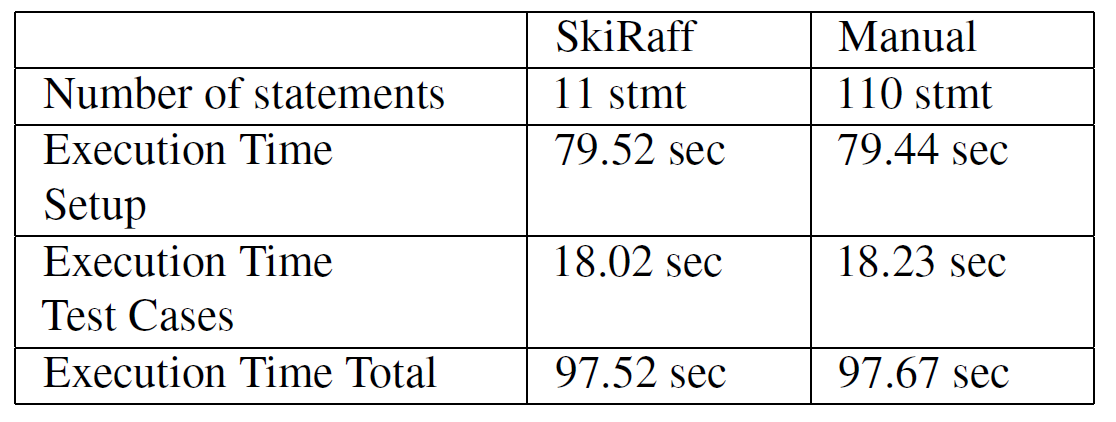
\includegraphics[width=1\textwidth]{figures/EvalResults.png}
        \caption{Results af evaluering med 10000 rækker i hver tabel udover CountryDim}
        \label{Results of evaluation}
    \end{figure}
\end{frame}

\subsection{Alternativer}
\begin{frame}{Metrikker}{}
Statiske
  \begin{itemize}
    \item<1-> \textbf{Statements}
    \item<2-> Fog index
    \item<3-> Cyclomatic complexity
  	\end{itemize}

\pause
\pause
\pause
Dynamiske
  \begin{itemize}
    \item<4-> \textbf{Runtime}
    \item<5-> Bug Count
  	\end{itemize}
\end{frame}


\begin{frame}{Usability Testing}{}
Udførsel
  \begin{itemize}
    \item<1-> Opskriv flere realistiske test planer
    \item<2-> Få ekspert brugere til at implementere planer med forskellige værktøjer:
	 \begin{itemize}
   	 \item<2-> SkiRaff
    	\item<2-> Manuel
    	\item<2-> QuerySurge
	\item<2-> AnyDBTest
  	\end{itemize}
   \item<3-> Fokuser på implementations hastighed og udsagn
  	\end{itemize}

\pause
\pause
\pause
Negativer
 \begin{itemize}
   \item<4-> Praktisk organisering
    \item<5-> Kvalitativ data kan også være svær at evaluere
    \item<6-> Store mængder data skal behandles
  \end{itemize}
\end{frame}


\section{Konklusion}
\begin{frame}{Konklusion}{}
  Hvad har vi lavet
  \begin{itemize}
    \item<1-> SkiRaff: Et framework til test af pygrametl programmer
    \item<2-> Dækker mange forskellige test cases med predicate klasserne
    \item<3-> Tests behøver færre linjer, men udføres med samme hastighed ift. manuel test
  \end{itemize}
\pause
\pause
\pause
Perspektiv
  \begin{itemize}
    \item<4-> Business Intelligence i moderne sammenhæng
    \item<5-> SkiRaff og ETL udvikling
  \end{itemize}


\end{frame}